\documentclass{standalone}
\usepackage{tikz}
\usepackage{xcolor}

\newcommand{\innerline}[1]{\if#112\else1\fi}

\definecolor{0}{rgb}{0.98, 0.96, 0.96} % white
\definecolor{1}{rgb}{0.40, 0.36, 0.38} % grey
\definecolor{2}{rgb}{0.06, 0.05, 0.03} % black

\begin{document}
    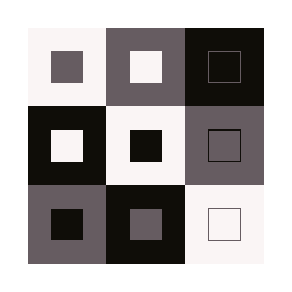
\begin{tikzpicture}
        \pgfmathsetmacro{\i}{0};
        \pgfmathsetmacro{\j}{0};
        \foreach[remember=\i as \i,remember=\j as \j] \outer/\inner in {0/1,1/0,2/2,2/0,0/2,1/1,1/2,2/1,0/0}{
            \begin{scope}[shift={(\i,\j)}]
                \draw[draw=none,fill=\outer] (0,0) rectangle (1,1);
                \if\outer\inner
                    \draw[draw=\innerline{\inner},fill=\inner] (0.3,0.3) rectangle (0.7,0.7);
                \else
                    \draw[draw=none,fill=\inner] (0.3,0.3) rectangle (0.7,0.7);
                \fi
            \end{scope}
            \if\i2
                \pgfmathtruncatemacro{\i}{0}; % CR
                \pgfmathtruncatemacro{\j}{\j-1}; % LF
            \else
                \pgfmathtruncatemacro{\i}{\i+1};
            \fi
        }
    \end{tikzpicture}
\end{document}